% !TeX encoding = UTF-8
% !TeX spellcheck = uk_UA
% !Mode:: "TeX:ACP"
\documentclass{KnuBulletin}

%% LaTeX/XeTeX шаблон для статтей у Вісник Київського національного університету імені Тараса Шевченка, 
%% Серія фізико-математичні науки.
%% 
%% Остання версія шаблону завжди тут: https://github.com/ertong/knu-bulletin
%% 
%% Автор: Ігор Литвиненко

\begin{document}

% Вказуємо рік  та номер виданння
\yearNumber{2014}{1}

% Вказуємо дату подачі до друку
\submittedDate{09.01.14}

% Вказуємо авторів. Цей блок повторюється для кожного автора.
% вказуючи науковий ступінь та вчене звання, 
% використовуйте такі скорочення: 
% д.ф.-м.н., к.ф.-м.н., проф., доц., асист., пров.н.с., с.н.с., м.н.с., аспірант
\author
{І. O. Іваненко} %Ініціали та прізвище
{аспірант} % науковий ступінь та вчене звання
{Київський національний університет імені Тараса Шевченка, 03680, м. Київ, пр-т Глушкова 4д} % назва та адреса установи
{I. O. Ivanenko}
{PhD student}
{Taras Shevchenko National University of Kyiv, 03680, Kyiv, Glushkova av., 4d}
{ivan@example.ua} % електронна адреса

\author
{І. І. Петренко}
{д.ф.-м.н., проф.}
{Київський національний університет імені Тараса Шевченка, 03680, м. Київ, пр-т Глушкова 4д}
{I. I. Petrenko}
{Doctor of Sciences, Full Professor}
{Taras Shevchenko National University of Kyiv, 03680, Kyiv, Glushkova av., 4d}
{petro@example.ua}

\header
{519.21} %УДК
% Назва статті українською мовою
{Зразок оформлення статті}
% Аннотація українською мовою
{
    В статті досліджується система обслуговування з рекурентним потоком заявок, які обробляються декількома виконавцями. Кожна заявка потребує експоненціального часу виконання з параметром, що залежить від типу заявки.

    В результаті, було описано спосіб знаходження стаціонарних ймовірностей  системи обслуговування та наведено приклад оптимізації параметрів вхідних потоків процесу з метою ефективного завантаження наявних виконавців. 
}
% ключові слова
{система обслуговування, рекурентний потік, стаціонарні ймовірності}
% теж саме англійською мовою
{Optimization of the queuing system with many servers and with recurrent flow\\}
{
    This paper considers a queuing system with recurrent flow of job and several servers. Every job requires exponential serving time with parameter depending on the type of the job. 
    
    As a result it was described a way to find the stationary probabilities of the service process. Finally, it was provided an example of input flow optimization problem in order to make servers to be loaded effectively.
    \\
}
{queuing system, recurrent flow, stationary probabilities}

%статтю може представляти лише член редколегії журналу
Статтю представив д.ф.-м.н., проф. Сидоренко М.М. 

\begin{multicols}{2}
    \noindent

    Розглянемо систему обслуговування з $M$ виконавцями та одним потоком заявок, який є потоком відновлення, де інтервали часу між заявками мають функцію розподілу $F(x)$. Кожна заявка з ймовірністю $p_i$ ($i=1,2,\dots,N$) потребує для обробки одного виконавця на експоненціально розподілений час з параметром $\mu_i$. Якщо всі $M$ виконавців зайняті, заявка отримує відмову в обслуговуванні та губиться.
    
    Випадок з одним типом заявок розглянуто в роботі \cite{takacs1962}. Робота \cite{lebedev1999queuing} описує випадок з різними заявками але з пуассонівським потоком на вході. Випадок з двома типами заявок розглянуто в роботі \cite{Ert2013servers2}.
    В даній роботі узагальнюється результат роботи \cite{Ert2013servers2} на випадок декількох типів заявок, що потребують різний середній час для обслуговування.
    Опишемо роботу цієї системи випадковим процесом
    \begin{equation*}
    X(t) \in \left\{ (x_1,\dots,x_N): \sum_{i=1}^{N} x_i \le M,\ x_i \ge 0,\ x_i \in N \right\}
    \end{equation*}
    де $X_i(t)$ -- кількість виконавців, зайнятих заявками $i$-го типу в момент часу $t\ge0$.
    
    Позначимо $\tau_n$ --- час надходження $n$-ї заявки. Тоді ($\tau_{n+1}-\tau_{n}$) має функцію розподілу $F(x)$.
    
    Позначимо $\zeta_n=X(\tau_n-0)$. 
    Тобто $\zeta_n=(\zeta_n^1,\dots,\zeta_n^N)$ --- це стан системи безпосередньо перед надходженням $n$-ї заявки.

    Розглянемо
    \begin{gather*}
    A_{r_1,...,r_N}^{n}(s) = \E{ e^{-s \tau_{n}} \prod_{i=1}^N \dbinom{\zeta_{n}^i}{r_i}}
    \end{gather*}    
    Для подальшого аналізу нам потрібні декілька допоміжних тверджень.
    
    \begin{lemma}[\cite{takacs1962}]
        \label{lem:binom-expectation}
        Якщо $\xi(M,p)$ -- випадкова величина розподілена біноміально з параметрами $M$ та $p\in(0,1)$, матимемо
        \begin{gather*}
        \E{ \dbinom{M-\xi(M,p)}{r}}
        =\E{ \dbinom{\xi(M,1-p)}{r}}
        =(1-p)^r \dbinom{M}{r}
        \end{gather*}
    \end{lemma}

    \begin{lemma}\label{lem:revert-multi-bin-sum}
        Нехай $p_{k_1,\dots,k_N}$ -- деякий розподіл ймовірностей:
        \begin{gather*}
	        p_{k_1,\dots,k_N}\ge0, 
	        k_1,\dots,k_N=\overline{0,M}, \\
	        \sum_{i=1}^N k_i\le M,
	        \sum_{k_i\colon \sum_{i=1}^N k_i \le M} p_{k_1,\dots,k_N}=1
        \end{gather*}
        
        Якщо
        \begin{gather*}
        b_{r_1,\dots,r_N}
            =\sum_{k_i\colon k_i \ge r_i \wedge \sum_{i=1}^N k_i \le M} \prod_{i=1}^N \dbinom{k_i}{r_i} p_{k_1,\dots,k_n}
        \end{gather*}
        $(r_1,\dots,r_N)$-й біноміальний момент цього розподілу, тоді
        \begin{gather*}
            p_{k_1,\dots,k_n}=
            \sum_{r_i\colon r_i \ge k_i \wedge \sum_{i=1}^N r_i \le M} \prod_{i=1}^N (-1)^{r_i-k_i} \dbinom{r_i}{k_i}
            b_{r_1,\dots,r_n}    
        \end{gather*}
    \end{lemma}
    
    \begin{proof}
        Спочатку покажемо, що для довільних $d_k$ та $0\le r \le m$ з
        \begin{gather}
        \label{eq:revert-2-bin-sum:1d-1}
        c_r=\sum_{k=r}^m \dbinom{k}{r}d_k
        \end{gather}
        випливає 
        \begin{gather}
        \label{eq:revert-2-bin-sum:1d-2}
        d_k=\sum_{r=k}^m (-1)^{r-k} \dbinom{r}{k}c_r
        \end{gather}
        Підставивши вираз для $c_r$ в формулу для $d_k$, отримаємо
        \begin{gather*}
        d_k=\sum_{r=k}^m (-1)^{r-k} \dbinom{r}{k}
        \sum_{i=r}^m \dbinom{i}{r}d_i
        = \sum_{i=k}^m d_i
        \sum_{r=k}^i 
        (-1)^{r-k} \dbinom{r}{k} \dbinom{i}{r}
        \end{gather*}
        Для доведення 
        (\ref{eq:revert-2-bin-sum:1d-1})-(\ref{eq:revert-2-bin-sum:1d-2}) 
        достатньо показати, що 
        \begin{gather*}
        \sum_{r=k}^i (-1)^{r-k} \dbinom{r}{k} \dbinom{i}{r} 
        =\begin{cases}
        1,&i=k\\
        0,&i>k
        \end{cases}
        \end{gather*}
        Випадок $i=k$ є очевидним. Розглянемо випадок $i>k$.
        \begin{multline*}
        \sum_{r=k}^i (-1)^{r-k} \dbinom{i}{r}\dbinom{r}{k}
        =\sum_{r=k}^i (-1)^{r-k} \dbinom{i}{k}\dbinom{i-k}{r-k}
        =\\=
        \dbinom{i}{k}\sum_{r=0}^{i-k} (-1)^{r} \dbinom{i-k}{r}
        =\dbinom{i}{k}(1-1)^{i-k}=0
        \end{multline*}
        Отже маємо (\ref{eq:revert-2-bin-sum:1d-1})-(\ref{eq:revert-2-bin-sum:1d-2}) доведеним.
        %
        Тепер до
        \begin{multline*}
            b_{r_1,\dots,r_N}
            =\sum_{k_i\colon k_i \ge r_i \wedge \sum_{i=1}^N k_i \le M} \prod_{i=1}^N \dbinom{k_i}{r_i} p_{k_1,\dots,k_n}
            =\\=
            \sum_{k_1=r_1}^{M-r_2-\dots-r_N}
            \dbinom{k_1}{r_1} 
            \sum_{k_2=r_2}^{M-k_1-r_3-\dots-r_N}
            \dbinom{k_2}{r_2} 
            \cdots\\\cdots
            \sum_{k_{N-1}=r_{N-1}}^{M-k_1-\dots-k_{N-2}-r_N}
            \dbinom{k_{N-1}}{r_{N-1}} 
            \sum_{k_N=r_N}^{M-k_1-\dots-k_{N-1}}
            \dbinom{k_N}{r_N} 
            p_{k_1,k_2}
        \end{multline*}
        застосуємо N разів перетворення (\ref{eq:revert-2-bin-sum:1d-1})-(\ref{eq:revert-2-bin-sum:1d-2}), 
        з чого й отримаємо твердження леми.
    \end{proof}
    
    \begin{lemma}
        [{\cite[c.~212]{klimov1966}}]
        \label{lem:abel}
        Якщо для деякої послідовності $x_n$ існує $\lim_{n\rightarrow\infty} x_n = x$, тоді
        $$
        \lim_{w\rightarrow 1} (1-w)\sum_{i=0}^\infty x_i w^i
        =x
        $$
    \end{lemma}
    
    

\begin{theorem}
    \label{thm:recA}
    $A_{r_1,...,r_N}^{n+1}(s)$ задовольняють наступним співвідношенням
    \begin{gather*}
    A_{0,...,0}^{n}(s) =\left(\int_0^\infty e^{-sx}\ dF(x)\right)^{n}= \phi(s)^{n}
    \end{gather*}
    \begin{multline*}
    A_{r_1,...,r_N}^{n+1}(s)
    =\phi\left(s+\sum_{i=1}^N \mu_i r_i\right)
    \cdot\\\cdot
    \sum_{k=1}^N p_k
    \left(\vphantom{\sum_\sum}
    A_{r_1,...,r_N}^{n}(s)+
    A_{r_1,\dots,r_{k}-1,\dots,r_N}^{n}(s)
    -
    \right.\\\left.
    -
    \sum_{a_i: \sum_{i=1}^N a_i = M}
    \dbinom{a_k}{r_k-1}
    \frac{\prod_{j=1}^N \dbinom{a_j}{r_j}} {\dbinom{a_k}{r_k}}
    A_{a_1,...,a_N}^{n}(s)
    \right)
    \end{multline*}    
        
\end{theorem}
\begin{proof}
   	Розглянемо
    \begin{gather*}
        \E{ e^{-s \tau_{n+1}} \prod_{i=1}^N \dbinom{\zeta_{n+1}^i}{r_i} |
            \zeta_n=(a_1,\dots,a_N), \tau_{n+1}-\tau_n=x}
        =
    \end{gather*}
    \begin{multline*}        
        =
        e^{-s x}\E{ e^{-s \tau_{n}} | \zeta_n=(a_1,\dots,a_N)}
        \cdot\\\cdot
        \E{ \prod_{i=1}^N \dbinom{\zeta_{n+1}^i}{r_i}
            | \zeta_n=(a_1,\dots,a_N), \tau_{n+1}-\tau_n=x}
        =
    \end{multline*}
    \begin{multline*}        
        =
        e^{-s x}\E{ e^{-s \tau_{n}} | \zeta_n=(a_1,\dots,a_N)}
        \cdot\\\cdot
        \sum_{k=1}^N p_k
        {\rm E}
        \left\{
            \dbinom{\zeta_{n+1}^k}{r_k}
            \frac{
                \prod_{i=1}^N \dbinom{a_i - \xi(a_i,1-e^{-\mu_i x})}{r_i}
            }{
            \dbinom{a_k - \xi(a_k,1-e^{-\mu_k x})}{r_k}
        	}
        	\right.\\\left.
         	| \zeta_n=(a_1,\dots,a_N), \tau_{n+1}-\tau_n=x, \text{$n$-а заявка має тип $k$}
        \vphantom{\dbinom{}{}}
        \right\}          
    \end{multline*}
    де $\xi(k,p)$ -- випадкова величина розподілена біноміально з параметрами $k$ та $p\in(0,1)$.
    
    Перетворимо останній вираз, використовуючи лему \ref{lem:binom-expectation}. Отримаємо
    \begin{multline*}
    \E{ e^{-s \tau_{n+1}} \prod_{i=1}^N \dbinom{\zeta_{n+1}^i}{r_i} |
        \zeta_n=(a_1,\dots,a_N), \tau_{n+1}-\tau_n=x}
    =
    \end{multline*}
    \begin{multline*}        
    =
    e^{-sx}
    \E{ e^{-s \tau_{n}} | \zeta_n=(a_1,\dots,a_N)}
    \cdot\\\cdot
    \sum_{k=1}^N p_k
    \frac{
        \prod_{i=1}^N e^{-\mu_i x r_i} \dbinom{a_i}{r_i}
    }{
        e^{-\mu_k x r_k} \dbinom{a_k}{r_k}
    }
    e^{-\mu_k x r_k}
    d(a_k,r_k)
    =    
    \end{multline*}
    \begin{multline*}        
    =
    e^{-\left(s+\sum_{k=1}^{N}\mu_k r_k\right)}
    \E{ e^{-s \tau_{n}} | \zeta_n=(a_1,\dots,a_N)}
    \cdot\\\cdot
    \sum_{k=1}^N p_k
    \frac{
        \prod_{i=1}^N  \dbinom{a_i}{r_i}
    }{
    \dbinom{a_k}{r_k}
    }
    d(a_k,r_k)
    \end{multline*}
 
 
     де
     \begin{gather*}
     d(a_k,r_k)=
     \begin{cases}
     \dbinom{a_k+1}{r_k}, & \sum_{i=1}^N a_i < M\\
     \dbinom{a_k}{r_k}, & \sum_{i=1}^N a_i = M
     \end{cases}
     \end{gather*}
     
    
    Якщо час очікування заявки має функцію розподілу $F(x)$ та $\phi(s)=\int_0^\infty e^{-sx}\ dF(x)$, тоді
    
    
    \begin{multline*}
    \E{ e^{-s \tau_{n+1}} \prod_{i=1}^N \dbinom{\zeta_{n+1}^i}{r_i} |
        \zeta_n=(a_1,\dots,a_N)}
    =\\=
    \phi\left(s+\sum_{i=1}^N \mu_i r_i\right)\E{ e^{-s \tau_{n}} | \zeta_n=(a_1,\dots,a_N)}
    \cdot\\\cdot
    \sum_{k=1}^N p_k
    \frac{
        \prod_{i=1}^N \dbinom{a_i}{r_i}
    }{
    \dbinom{a_k}{r_k}
    }d(a_k,r_k)
    \end{multline*}
    Домножимо рівність на $\prob{\zeta_n=(a_1,\dots,a_N)}$ та просумуємо по $(a_1,\dots,a_N)\colon \sum_{i=1}^N a_i \le M$. Матимемо
    \begin{multline*}
    A_{r_1,...,r_N}^{n+1}(s)
    =\phi\left(s+\sum_{i=1}^N \mu_i r_i\right)
    \sum_{k=1}^N p_k
    \cdot\\\cdot
    \left(\sum_{a_i: 1+\sum_{i=1}^N a_i \le M}
    \frac{\prod_{j=1}^N \dbinom{a_j}{r_j}}{\dbinom{a_k}{r_k}}
    \left(\dbinom{a_k}{r_k}+\dbinom{a_k}{r_k-1}\right)
    \cdot
    \right.\\\left.
    \cdot
    \E{ e^{-s \tau_{n}} | \zeta_n=(a_1,\dots,a_N)}
    \prob{\zeta_n=(a_1,\dots,a_N)}
    +
    \right.\\\left.
    +
    \sum_{a_i: 1+\sum_{i=1}^N a_i > M}
    \prod_{j=1}^N \dbinom{a_j}{r_j}
    \E{ e^{-s \tau_{n}} | \zeta_n=(a_1,\dots,a_N)}
    \cdot
    \right.\\\left.
    \cdot
    \prob{\zeta_n=(a_1,\dots,a_N)}
    \vphantom{\sum^\sum}
    \right)
    \end{multline*}
    
    Враховуючи, що
    \begin{multline*}
    \label{eq:cond-expactation-multi}
    A_{r_1,...,r_N}^{n}(s)
    =
    \sum_{a_i: \sum_{i=1}^N a_i \le M}
    \prod_{i=1}^N \dbinom{a_i}{r_i}
    \cdot\\\cdot
    \E{ e^{-s \tau_{n}} | \zeta_n=(a_1,\dots,a_N)}
    \prob{\zeta_n=(a_1,\dots,a_N)}
    \end{multline*}
    та використавши лему \ref{lem:revert-multi-bin-sum}, отримаємо твердження
    теореми. 
\end{proof}    

    \begin{corollary}
        \label{thm:recPhi}        
        Генератрису для $A_{r_1,...,r_N}^{n}(s)$
        \begin{gather}
        \Phi_{r_1,...,r_N}(s,w) = \sum_{n=1}^{\infty} A_{r_1,...,r_N}^{n}(s) w^n
        \end{gather}
        можна визначити наступними співвідношеннями
        \begin{gather*}
        \Phi_{0,\dots,0}(s,w) 
        = \frac{w \phi(s)}{1-w \phi(s)}
        \end{gather*}
        \begin{multline*}
        \Phi_{r_1,...,r_N}(s,w)
        =
        \frac
        {w \phi\left(s+\sum_{i=1}^N \mu_i r_i\right)}
        {1- w \phi\left(s+\sum_{i=1}^N \mu_i r_i\right)}
        \cdot\\\cdot
        \left(\vphantom{\sum_\sum}
        \prod_{i=1}^N \dbinom{j_{0}^i}{r_i}
        +
        \sum_{k=1}^N p_k
        \left[\vphantom{\sum_\sum}
        \Phi_{r_1,\dots,r_{k}-1,\dots,r_N}(s,w)
        -
        \right.\right.\\\left.\left.
        -
        \sum_{a_i: \sum_{i=1}^N a_i = M}
        \Phi_{a_1,...,a_N}(s,w)
        \dbinom{a_k}{r_k-1}
        \frac{\prod_{j=1}^N \dbinom{a_j}{r_j}} {\dbinom{a_k}{r_k}}
        \right]
        \right)
        \end{multline*}
            
        де $j_{0}^i$ -- кількість зайнятих виконавців в момент часу $t=0$ заявками $i$-го типу.
    \end{corollary}
\begin{proof}
	\begin{multline*}
	  \Phi_{0,\dots,0}(s,w) 
	  = \sum_{n=1}^{\infty} A_{0,\dots,0}^{n}(s) w^n
	  =\\= 
	  \sum_{n=1}^{\infty} \phi(s)^n w^n
	  = \frac{w \phi(s)}{1-w \phi(s)}
	\end{multline*}
    Рекурентне співвідношення для $\Phi_{r_1,\dots,r_N}(s,w)$ отримується 
    перетворенням відповідного рекурентного співвідношення для $A_{r_1,\dots,r_N}^n(s)$,
    отриманого в теоремі \ref{thm:recA}.
    
    	Враховуючи, що
        \begin{gather*}
        A_{r_1,...,r_N}^{1}(s)
        =\int_{0}^{\infty}
        \E{e^{-s\tau_1} \prod_{i=1}^N \dbinom{\zeta_{1}^i}{r_i}|\tau_1=x} \ dx
        =\\=
        \int_{0}^{\infty} e^{-sx}
        \E{\prod_{i=1}^N e^{-\mu_i x r}\dbinom{\zeta_{0}^i}{r_i}|\tau_1=x} \ dx
        =\\=
        \phi\left(s+\sum_{i=1}^N \mu_i r_i\right)
        \prod_{i=1}^N \dbinom{j_{0}^i}{r_i}
        \end{gather*}
        матимемо
        \begin{multline*}
        \Phi_{r_1,...,r_N}(s,w)
        - w \phi\left(s+\sum_{i=1}^N \mu_i r_i\right)
        \prod_{i=1}^N \dbinom{j_{0}^i}{r_i}
        =\\=
        w\phi\left(s+\sum_{i=1}^N \mu_i r_i\right)
        \sum_{k=1}^N p_k
        \left(\vphantom{\sum_\sum}
        \Phi_{r_1,...,r_N}(s,w)
        +
        \right.\\\left.
        +
        \Phi_{r_1,\dots,r_{k}-1,\dots,r_N}(s,w)
        %\right.\\\left.
        -
        \right.\\\left.
        -
        \sum_{a_i: \sum_{i=1}^N a_i = M}
        \dbinom{a_k}{r_k-1}
        \frac{\prod_{j=1}^N \dbinom{a_j}{r_j}} {\dbinom{a_k}{r_k}}
        \Phi_{a_1,...,a_N}(s,w)
        \right)
        \end{multline*}
        
        \begin{multline*}
        \Phi_{r_1,...,r_N}(s,w)
        =
        \frac
        {w \phi\left(s+\sum_{i=1}^N \mu_i r_i\right)}
        {1- w \phi\left(s+\sum_{i=1}^N \mu_i r_i\right)}
        \cdot
        \\
        \cdot
        \left(
        \prod_{i=1}^N \dbinom{j_{0}^i}{r_i}
        +
        \sum_{k=1}^N p_k
        \left[\vphantom{\sum_\sum}
        \Phi_{r_1,\dots,r_{k}-1,\dots,r_N}(s,w)
        -
        \right.\right.\\\left.\left.
        -
        \sum_{a_i: n_k+\sum_{i=1}^N a_i > M}
        \dbinom{a_k}{r_k-1}
        \frac{\prod_{j=1}^N \dbinom{a_j}{r_j}} {\dbinom{a_k}{r_k}}
        \Phi_{a_1,...,a_N}(s,w)
        \right]
        \right)
        \end{multline*}
        
        \begin{multline*}
        \Phi_{r_1,...,r_N}(s,w)
        =
        \frac
        {w \phi\left(s+\sum_{i=1}^N \mu_i r_i\right)}
        {1- w \phi\left(s+\sum_{i=1}^N \mu_i r_i\right)}
        \cdot
        \\
        \cdot
        \left(\vphantom{\sum_\sum}
        \prod_{i=1}^N \dbinom{j_{0}^i}{r_i}
        +
        \sum_{k=1}^N p_k
        \left[\vphantom{\sum_\sum}
        \Phi_{r_1,\dots,r_{k}-1,\dots,r_N}(s,w)
        -
        \right.\right.\\\left.\left.
        -
        \sum_{a_j: \sum_{j=1}^N a_j = M}
        \Phi_{a_1,...,a_N}(s,w)
        \dbinom{a_k}{r_k-1}
        \frac{\prod_{j=1}^N \dbinom{a_j}{r_j}} {\dbinom{a_k}{r_k}}
        \right]
        \right)
        \end{multline*}
        Що і треба було довести.
\end{proof}





\begin{theorem}
    \label{thm:lim-bin-mom-recurrent}
    Біноміальні моменти
   	\begin{gather*}
        B_{r_1,\dots,r_N}
        = \sum_{a_i: \sum_{i=1}^N a_i \le M}
        \prod_{i=1}^N \dbinom{a_i}{r_i}
        P_{a_1,\dots,a_N}
    \end{gather*}
    стаціонарного розподілу
    \begin{gather*}
    P_{a_1,\dots,a_N} 
    = \lim_{n\rightarrow\infty} \prob{\zeta_n=(a_1,\dots,a_N)}
    \end{gather*}
    процесу $\zeta_n=(\zeta_n^1,\dots,\zeta_n^N)$
    задовольняють наступним співвідношенням:
	\begin{gather*}
    B_{0,\dots,0}=1
    \end{gather*}
    \begin{multline*}
        B_{r_1,\dots,r_N}=
        \frac
        { \phi\left(\sum_{i=1}^N \mu_i r_i\right)}
        {1- \phi\left(\sum_{i=1}^N \mu_i r_i\right)}
        \cdot\\\cdot
        \left(\vphantom{\sum_\sum}
        \sum_{k=1}^N p_k
        \left[\vphantom{\sum_\sum}
        B_{r_1,\dots,r_{k}-1,\dots,r_N}
        %\right.\right.\\\left.\left.
        -
        \right.\right.\\\left.\left.
        -
        \sum_{a_j: \sum_{j=1}^N a_j = M}
        B_{a_1,...,a_N}
        \dbinom{a_k}{r_k-1}
        \frac{\prod_{j=1}^N \dbinom{a_j}{r_j}} {\dbinom{a_k}{r_k}}
        \right]
        \right)
    \end{multline*}    
\end{theorem}
\begin{proof}
    Використовуючи лему \ref{lem:abel}, маємо
    \begin{multline*}
    B_{r_1,...,r_N}
    =\lim_{n\rightarrow\infty} B_{r_1,...,r_N}^{n}
    =\\=
    \lim_{w\rightarrow 1} (1-w)\sum_{i=1}^\infty B_{r_1,...,r_N}^{i}w^i 
    =\lim_{w\rightarrow 1} (1-w)\Phi_{r_1,...,r_N}(0,w)
    \end{multline*}
        
    Використовуючи рекурентне співвідношення для $\Phi_{r_1,\dots,r_N}(0,w)$
    з наслідку \ref{thm:recPhi}, маємо
    \begin{multline*}
    \lim_{w\rightarrow 1} (1-w)\Phi_{r_1,...,r_N}(w)
    =
    \frac
    { \phi\left(\sum_{i=1}^N \mu_i r_i\right)}
    {1- \phi\left(\sum_{i=1}^N \mu_i r_i\right)}
    \cdot\\\cdot
    \left(\vphantom{\sum_\sum}
    \sum_{k=1}^N p_k
    \left[\vphantom{\sum_\sum}
    \lim_{w\rightarrow 1} (1-w) \Phi_{r_1,\dots,r_{k}-1,\dots,r_N}(w)
    -
    \right.\right.\\\left.\left.
    -
    \sum_{a_j: \sum_{j=1}^N a_j = M}
    \lim_{w\rightarrow 1} (1-w) \Phi_{a_1,...,a_N}(w)
    \cdot
    \right.\right.\\\left.\left.
    \cdot
    \dbinom{a_k}{r_k-1}
    \frac{\prod_{j=1}^N \dbinom{a_j}{r_j}} {\dbinom{a_k}{r_k}}
    \right]
    \right)
    \end{multline*}
    звідки отримуємо рекурентне співвідношення для $B_{r_1,\dots,r_N}$. 
    
    Розглянемо випадок $B_{0,0}$ окремо.        
    \begin{multline*}
    \lim_{w\rightarrow 1} (1-w) \Phi_{0,\dots,0}(w) 
    = \lim_{w\rightarrow 1} \frac{(1-w) w \phi(0)}{1-w \phi(0)}
    = \\ =
    \lim_{w\rightarrow 1} \frac{(1-w) w \int_0^\infty e^{-0x}\ dF(x)}{1-w \int_0^\infty e^{-0x}\ dF(x)}  
    = \lim_{w\rightarrow 1} \frac{(1-w) w}{1-w}  
    = \\ =
    \lim_{w\rightarrow 1} w 
    =1
    \end{multline*}
    
    Теорему доведено.
\end{proof}


    \begin{lemma}
        \label{lem:rec}
        Якщо $f(0,\dots,0)=0$, то розв'язок рекурентного співвідношення
        \begin{multline*}
        b_{r_1,\dots,r_N}
        = c(r_1,\dots,r_N)
        \cdot\\\cdot
        \sum_{i=1}^{N} c_i b_{r_1,\dots,r_i-1,\dots,r_N}
        + f(r_1,\dots,r_N)
        \end{multline*}
        
        можна подати у вигляді
        \begin{multline}
            \label{eq:lem:rec:solution}
            b_{r_1,\dots,r_N}
            = 
            d_{0,\dots,0,r_1,\dots,r_N}
            c_1^{r_1}\cdots
            c_N^{r_N}
            b_{0,\dots,0}
            \cdot\\\cdot
            \sum_{a_1=0}^{r_1}
            \cdots
            \sum_{a_N=0}^{r_N}
            d_{a_1,\dots,a_N,r_1,\dots,r_N}
            f(a_1,\dots,a_N)
            \cdot\\\cdot
            c_1^{r_1-a_1}
            \cdots
            c_N^{r_N-a_N}
        \end{multline}        
        де
        \iffalse
            \begin{gather*}
            d_{a_1,\dots,a_N,a_1,\dots,a_N}=1\\
            %d_{a_1,\dots,a_2,a_1,\dots,r_2}=c(a_1,r_2)d_{a_1,a_2,a_1,r_2-1}  \\
            %d_{a_1,\dots,a_2,r_1,\dots,a_2}=c(r_1,a_2)d_{a_1,a_2,r_1-1,a_2}  \\
            d_{a_1,\dots,a_N,r_1,\dots,r_N}=c(r_1,\dots,r_N)
            \sum_{i=1}^{N}d_{a_1,\dots,a_N,r_1,\dots,r_i-1,\dots,r_N}
            \end{gather*}            
        \fi
        \begin{multline*}
            d_{a_1,\dots,a_N,r_1,\dots,r_N}
            =\\=
            \begin{cases}
                c(r_1,\dots,r_N)
                \cdot\\\cdot
                \sum_{i=1}^{N}d_{a_1,\dots,a_N,r_1,\dots,r_i-1,\dots,r_N},
                & a_i, r_i \ge 0,  i=\overline{1,N}\\
                %
                1, & a_i=r_i, i=\overline{1,N}\\
                0, &else
            \end{cases}
        \end{multline*}            
        
        тобто
        \begin{multline*}
        d_{a_1,\dots,a_N,r_1,\dots,r_N}
        =
        \sum_{\text{по всім шляхам $\pi$}\atop \text{з $(a_1,\dots,a_N)$ в $(r_1,\dots,r_N)$}}
        \\
        \prod_{\text{по всіх клітинках $(b_1,\dots,b_N)$}\atop\text{ шляху $\pi$ крім $(a_1,\dots,a_N)$}}
        c(b_1,\dots,b_N)
        \end{multline*}            
    \end{lemma}
    \begin{proof}
        
    Доведення леми можна отримати підстановкою (\ref{eq:lem:rec:solution})  у рекурентне співвідношення для $b_{r_1,\dots,r_N}$.
        
        \begin{multline*}
        d_{0,\dots,0,r_1,\dots,r_N}
        c_1^{r_1}\cdots
        c_N^{r_N}
        b_{0,\dots,0}
        +\\+
        \sum_{a_1=0}^{r_1}
        \cdots
        \sum_{a_N=0}^{r_N}
        d_{a_1,\dots,a_N,r_1,\dots,r_N}
        f(a_1,\dots,a_N)
        \cdot\\\cdot
        c_1^{r_1-a_1}
        \cdots
        c_N^{r_N-a_N}
        =
        \end{multline*}
        \begin{multline*}
        =
        f(r_1,\dots,r_N) + 
        \left(
        c_1^{r_1}
        \cdots
        c_N^{r_N}
        b_{0,\dots,0}
        c(r_1,\dots,r_N) 
        \cdot\right.\\\left.\cdot
        \sum_{i=1}^{N}
        d_{0,\dots,0,r_1,\dots,r_i-1,\dots,r_N}
        +        
        \right.\\\left.
        +
        \sum_{i=1}^{N}
        \sum_{a_1=0}^{r_1}
        \cdots
        \sum_{a_i=0}^{r_i-1}
        \cdots
        \sum_{a_N=0}^{r_N}
        c(r_1,\dots,r_N) 
        \cdot\right.\\\left.\cdot
        d_{a_1,\dots,a_N,r_1,\dots,r_i-1,\dots,r_N}
        f(a_1,\dots,a_N)
        c_1^{r_1-a_1}
        \cdots
        c_N^{r_N-a_N}
        \right)
        \end{multline*}        
        
        Залишається довести тотожність
        \begin{multline*}
        \sum_{a_1=0}^{r_1}
        \cdots
        \sum_{a_N=0}^{r_N}
        d_{a_1,\dots,a_N,r_1,\dots,r_N}
        f(a_1,\dots,a_N)
        \cdot\\\cdot
        c_1^{r_1-a_1}
        \cdots
        c_N^{r_N-a_N}
        =
        \end{multline*}
        \begin{multline*}
        =
         f(r_1,\dots,r_N) 
        +
        \sum_{i=1}^{N}
        \sum_{a_1=0}^{r_1}
        \cdots
        \sum_{a_i=0}^{r_i-1}
        \cdots
        \sum_{a_N=0}^{r_N}
        c(r_1,\dots,r_N) 
        \cdot\\\cdot
        d_{a_1,\dots,a_N,r_1,\dots,r_i-1,\dots,r_N}
        f(a_1,\dots,a_N)
        c_1^{r_1-a_1}
        \cdots
        c_N^{r_N-a_N}
        \end{multline*}        
        
        Зауважимо, що з означення можна показати
        \begin{gather*}
        d_{a_1,\dots,a_N,r_1,\dots,r_N}=0, \text{якщо існує}\ i: a_i>r_i
        \end{gather*}
        
        Тому, додаючи необхідні нульові доданки та знаючи, що         $d_{r_1,\dots,r_N,r_1,\dots,r_N}=1$, матимемо
        \begin{multline*}
        f(r_1,\dots,r_N) + 
        \sum_{i=1}^{N}
        \sum_{a_1=0}^{r_1}
        \cdots
        \sum_{a_i=0}^{r_i-1}
        \cdots
        \sum_{a_N=0}^{r_N}
        c(r_1,\dots,r_N) 
        \cdot\\\cdot
        d_{a_1,\dots,a_N,r_1,\dots,r_i-1,\dots,r_N}
        \cdot\\\cdot
        f(a_1,\dots,a_N)
        c_1^{r_1-a_1}
        \cdots
        c_N^{r_N-a_N}
        =
        \end{multline*}
        \begin{multline*}
        =
        \sum_{a_1=0}^{r_1}
        \cdots
        \sum_{a_N=0}^{r_N}
        \sum_{i=1}^{N}
        c(r_1,\dots,r_N) 
        \cdot\\\cdot
        d_{a_1,\dots,a_N,r_1,\dots,r_i-1,\dots,r_N}
        \cdot\\\cdot
        f(a_1,\dots,a_N)
        c_1^{r_1-a_1}
        \cdots
        c_N^{r_N-a_N}
        =
        \end{multline*}
        \begin{multline*}
        =
        \sum_{a_1=0}^{r_1}
        \cdots
        \sum_{a_N=0}^{r_N}
        d_{a_1,\dots,a_N,r_1,\dots,r_N}
        f(a_1,\dots,a_N)
        \cdot\\\cdot
        c_1^{r_1-a_1}
        \cdots
        c_N^{r_N-a_N}
        \end{multline*}        
        Що і треба було довести.
        
        
    \end{proof}

    \begin{corollary}
        Біноміальні моменти
        \begin{gather*}
        B_{r_1,\dots,r_N}
        = \sum_{a_i: \sum_{i=1}^N a_i \le M}
        \prod_{i=1}^N \dbinom{a_i}{r_i}
        P_{a_1,\dots,a_N}
        \end{gather*}
        стаціонарного розподілу
        \begin{gather*}
        P_{a_1,\dots,a_N} 
        = \lim_{n\rightarrow\infty} \prob{\zeta_n=(a_1,\dots,a_N)}
        \end{gather*}
        процесу $\zeta_n=(\zeta_n^1,\dots,\zeta_n^N)$
        можна подати у вигляді:
       
        \begin{multline*}
            \label{eq:thm:binom-rec:1}
            B_{r_1,\dots,r_N}
            = 
            d_{0,\dots,0,r_1,\dots,r_N}
            p_1^{r_1}\cdots
            p_N^{r_N}
            -\\-
            \sum_{b_1=0}^{r_1}
            \cdots
            \sum_{b_N=0}^{r_N}
            d_{b_1,\dots,b_N,r_1,\dots,r_N}
            p_1^{r_1-a_1}
            \cdots
            p_N^{r_N-a_N}
            \cdot\\\cdot
            c(b_1,\dots,b_N)
            \sum_{a_j: \sum_{j=1}^N a_j = M}
            \sum_{k=1}^N p_k
            B_{a_1,...,a_N}
            \cdot\\\cdot
            \dbinom{a_k}{r_k-1}
            \frac{\prod_{j=1}^N \dbinom{a_j}{r_j}} {\dbinom{a_k}{r_k}}
        \end{multline*} 
        
        де $d_{b_1,b_2,r_1,r_2}$ визначені як в лемі \ref{lem:rec} при
        \begin{gather*}
        c(r_1,\dots,r_N)=
        \frac
        { \phi\left(\sum_{i=1}^N \mu_i r_i\right)}
        {1- \phi\left(\sum_{i=1}^N \mu_i r_i\right)}        
        \end{gather*}
        та $B_{a_1,\dots,a_N}$ для $a_j: \sum_{j=1}^N a_j = M$ визначені системою 
        відповідних рівнянь (\ref{eq:thm:binom-rec:1}) (якщо її розв'язок існує).
    \end{corollary}
    \begin{proof}
        Застосовуємо лему \ref{lem:rec} до результату теореми \ref{thm:lim-bin-mom-recurrent}.
    \end{proof}
    
    
    \begin{lemma}
        Якщо $P_{r_1,\dots,r_N}$ стаціонарні ймовірності для процесу 
        $\zeta_n$.
        Тоді стаціонарні ймовірності $\overline{P}_{r_1,\dots,r_N}$ процесу $X(\tau_n)$, $n=0,1,\dots$ дорівнюють
        \begin{multline}
        \label{eq:X:stat:prob}
        \overline{P}_{r_1,\dots,r_N}
        =\\=
        \begin{cases}
        \sum_{i=1}^N P_{r_1,\dots,r_i-1,\dots,r_2} p_i, & \sum_{i=1}^N r_i<M, \\
        \sum_{i=1}^N P_{r_1,\dots,r_i-1,\dots,r_2} p_i+P_{r_1,\dots,r_N}, & \sum_{i=1}^N r_i=M.
        \end{cases}
        \end{multline}
    \end{lemma}

    Розглянемо задачу оптимізації параметрів $p_1,\dots,p_N$  вхідного потоку
    \begin{gather*}
    \begin{cases}
        \sum_{i=1}^{N} c_i \E{X^i} \rightarrow max,\\
        \sum_{i=1}^{N} p_i=1,
    \end{cases}
    \end{gather*}
    де розподіл вектора $(X^1,\dots,X^N)$ співпадає з (\ref{eq:X:stat:prob}).
    \begin{gather*}
        \E{X^i} = \sum_{a:a_1+\cdots+a_n \le M} 
        \overline{P}_{a_1,\dots,a_N}(p_1,\dots,p_n) a_i
    \end{gather*}
        
    Матимемо
    \begin{gather*}
        \begin{cases}
            \sum_{a:a_1+\cdots+a_n \le M} 
            \overline{P}_{a_1,\dots,a_N}(p_1,\dots,p_n)
            \sum_{i=1}^{N} 
            c_i 
            a_i \rightarrow max,\\
            \sum_{i=1}^{N} p_i=1,
        \end{cases}
    \end{gather*}

    Дану задачу оптимізації можна розв'язати чисельно.
    Розглянемо, для прикладу, випадок системи з параметрами
    $\mu=(0.34, 0.68, 0.136)$ та
    $c=(260, 311, 400)$, 
    якщо час між надходженнями заявок розподілений згідно гамма розподілу з параметрами $2$ та $1/3$.
    
    \begin{figure}[H]
        \hfil
        % This file was created by matlab2tikz v0.3.3.
% Copyright (c) 2008--2013, Nico Schlömer <nico.schloemer@gmail.com>
% All rights reserved.
% 
% The latest updates can be retrieved from
%   http://www.mathworks.com/matlabcentral/fileexchange/22022-matlab2tikz
% where you can also make suggestions and rate matlab2tikz.
% 
% 
% 
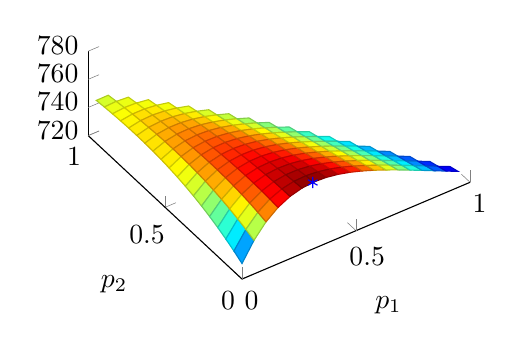
\begin{tikzpicture}

\begin{axis}[%
width=0.4\textwidth,
height=0.34\textwidth,
unbounded coords=jump,
view={-34}{64},
scale only axis,
xmin=0,
xmax=1,
xlabel={$p_1$},
ymin=0,
ymax=1,
ylabel={$p_2$},
zmin=720,
zmax=780,
title={},
axis x line*=bottom,
axis y line*=left,
axis z line*=left
]

\addplot3[%
surf,
colormap/jet,
shader=faceted,
draw=black,
mesh/rows=20]
table[row sep=crcr,header=false] {
0 0 731.013477419278\\
0 0.0526315789473684 734.563492038168\\
0 0.105263157894737 737.729408392122\\
0 0.157894736842105 740.528468106508\\
0 0.210526315789474 742.978554038338\\
0 0.263157894736842 745.09789642451\\
0 0.315789473684211 746.904825958476\\
0 0.368421052631579 748.417569122293\\
0 0.421052631578947 749.654081141013\\
0 0.473684210526316 750.631912084126\\
0 0.526315789473684 751.368101880567\\
0 0.578947368421053 751.879100311183\\
0 0.631578947368421 752.180708372434\\
0 0.684210526315789 752.288037749064\\
0 0.736842105263158 752.215485477769\\
0 0.789473684210526 751.976721218005\\
0 0.842105263157895 751.584684863127\\
0 0.894736842105263 751.051592520235\\
0 0.947368421052632 750.388949157829\\
0 1 749.607566465488\\
0.0526315789473684 0 743.913171185566\\
0.0526315789473684 0.0526315789473684 746.315283932909\\
0.0526315789473684 0.105263157894737 748.388322245117\\
0.0526315789473684 0.157894736842105 750.150557819217\\
0.0526315789473684 0.210526315789474 751.620150968364\\
0.0526315789473684 0.263157894736842 752.814986281177\\
0.0526315789473684 0.315789473684211 753.752540898407\\
0.0526315789473684 0.368421052631579 754.449781247862\\
0.0526315789473684 0.421052631578947 754.923084370203\\
0.0526315789473684 0.473684210526316 755.188180291501\\
0.0526315789473684 0.526315789473684 755.260112235672\\
0.0526315789473684 0.578947368421053 755.153211807271\\
0.0526315789473684 0.631578947368421 754.881086602822\\
0.0526315789473684 0.684210526315789 754.456618019832\\
0.0526315789473684 0.736842105263158 753.891967322244\\
0.0526315789473684 0.789473684210526 753.198588286934\\
0.0526315789473684 0.842105263157895 752.387244996573\\
0.0526315789473684 0.894736842105263 751.468033559872\\
0.0526315789473684 0.947368421052632 750.450406731602\\
0.0526315789473684 1 Inf\\
0.105263157894737 0 753.409380564311\\
0.105263157894737 0.0526315789473684 754.834848575162\\
0.105263157894737 0.105263157894737 755.987076733252\\
0.105263157894737 0.157894736842105 756.883470859558\\
0.105263157894737 0.210526315789474 757.540924609301\\
0.105263157894737 0.263157894736842 757.9757423033\\
0.105263157894737 0.315789473684211 758.203582455857\\
0.105263157894737 0.368421052631579 758.239418850639\\
0.105263157894737 0.421052631578947 758.097516346414\\
0.105263157894737 0.473684210526316 757.791418915431\\
0.105263157894737 0.526315789473684 757.333947721857\\
0.105263157894737 0.578947368421053 756.737207331604\\
0.105263157894737 0.631578947368421 756.012598405466\\
0.105263157894737 0.684210526315789 755.170835463672\\
0.105263157894737 0.736842105263158 754.221968521654\\
0.105263157894737 0.789473684210526 753.175407584744\\
0.105263157894737 0.842105263157895 752.039949154881\\
0.105263157894737 0.894736842105263 750.823804046816\\
0.105263157894737 0.947368421052632 Inf\\
0.105263157894737 1 Inf\\
0.157894736842105 0 760.025520507465\\
0.157894736842105 0.0526315789473684 760.642309621724\\
0.157894736842105 0.105263157894737 761.037811768447\\
0.157894736842105 0.157894736842105 761.227613636655\\
0.157894736842105 0.210526315789474 761.226618759984\\
0.157894736842105 0.263157894736842 761.04902405895\\
0.157894736842105 0.315789473684211 760.708308401317\\
0.157894736842105 0.368421052631579 760.217231028797\\
0.157894736842105 0.421052631578947 759.587837976169\\
0.157894736842105 0.473684210526316 758.831474864116\\
0.157894736842105 0.526315789473684 757.958804678408\\
0.157894736842105 0.578947368421053 756.979829355574\\
0.157894736842105 0.631578947368421 755.903914179461\\
0.157894736842105 0.684210526315789 754.739814155319\\
0.157894736842105 0.736842105263158 753.495701669827\\
0.157894736842105 0.789473684210526 752.179194868389\\
0.157894736842105 0.842105263157895 750.797386286963\\
0.157894736842105 0.894736842105263 Inf\\
0.157894736842105 0.947368421052632 Inf\\
0.157894736842105 1 Inf\\
0.210526315789474 0 764.261011630062\\
0.210526315789474 0.0526315789473684 764.222410079989\\
0.210526315789474 0.105263157894737 764.008394842627\\
0.210526315789474 0.157894736842105 763.632378290111\\
0.210526315789474 0.210526315789474 763.107056106864\\
0.210526315789474 0.263157894736842 762.444413989388\\
0.210526315789474 0.315789473684211 761.655740597323\\
0.210526315789474 0.368421052631579 760.751645394874\\
0.210526315789474 0.421052631578947 759.74208022469\\
0.210526315789474 0.473684210526316 758.636363636759\\
0.210526315789474 0.526315789473684 757.443207153784\\
0.210526315789474 0.578947368421053 756.170742793436\\
0.210526315789474 0.631578947368421 754.826551288446\\
0.210526315789474 0.684210526315789 753.417690549422\\
0.210526315789474 0.736842105263158 751.95072400427\\
0.210526315789474 0.789473684210526 750.431748523806\\
0.210526315789474 0.842105263157895 Inf\\
0.210526315789474 0.894736842105263 Inf\\
0.210526315789474 0.947368421052632 Inf\\
0.210526315789474 1 Inf\\
0.263157894736842 0 766.564287743779\\
0.263157894736842 0.0526315789473684 766.004044958114\\
0.263157894736842 0.105263157894737 765.307521938997\\
0.263157894736842 0.157894736842105 764.485948467819\\
0.263157894736842 0.210526315789474 763.549878484692\\
0.263157894736842 0.263157894736842 762.509211692925\\
0.263157894736842 0.315789473684211 761.373217854162\\
0.263157894736842 0.368421052631579 760.150562971807\\
0.263157894736842 0.421052631578947 758.849336696313\\
0.263157894736842 0.473684210526316 757.477080403912\\
0.263157894736842 0.526315789473684 756.04081550215\\
0.263157894736842 0.578947368421053 754.547071602796\\
0.263157894736842 0.631578947368421 753.001914276959\\
0.263157894736842 0.684210526315789 751.410972170057\\
0.263157894736842 0.736842105263158 749.779463307127\\
0.263157894736842 0.789473684210526 Inf\\
0.263157894736842 0.842105263157895 Inf\\
0.263157894736842 0.894736842105263 Inf\\
0.263157894736842 0.947368421052632 Inf\\
0.263157894736842 1 Inf\\
0.315789473684211 0 767.322683942097\\
0.315789473684211 0.0526315789473684 766.354055408307\\
0.315789473684211 0.105263157894737 765.281743009781\\
0.315789473684211 0.157894736842105 764.114965619516\\
0.315789473684211 0.210526315789474 762.862341630027\\
0.315789473684211 0.263157894736842 761.531916264914\\
0.315789473684211 0.315789473684211 760.1311895341\\
0.315789473684211 0.368421052631579 758.66714439548\\
0.315789473684211 0.421052631578947 757.146274771053\\
0.315789473684211 0.473684210526316 755.574613138236\\
0.315789473684211 0.526315789473684 753.95775747859\\
0.315789473684211 0.578947368421053 752.300897417921\\
0.315789473684211 0.631578947368421 750.608839434991\\
0.315789473684211 0.684210526315789 748.886031051945\\
0.315789473684211 0.736842105263158 Inf\\
0.315789473684211 0.789473684210526 Inf\\
0.315789473684211 0.842105263157895 Inf\\
0.315789473684211 0.894736842105263 Inf\\
0.315789473684211 0.947368421052632 Inf\\
0.315789473684211 1 Inf\\
0.368421052631579 0 766.862125010563\\
0.368421052631579 0.0526315789473684 765.579030561661\\
0.368421052631579 0.105263157894737 764.21894003708\\
0.368421052631579 0.157894736842105 762.789309998627\\
0.368421052631579 0.210526315789474 761.297082933231\\
0.368421052631579 0.263157894736842 759.748715123388\\
0.368421052631579 0.315789473684211 758.150204082487\\
0.368421052631579 0.368421052631579 756.507115342442\\
0.368421052631579 0.421052631578947 754.824608431576\\
0.368421052631579 0.473684210526316 753.107461923022\\
0.368421052631579 0.526315789473684 751.360097469014\\
0.368421052631579 0.578947368421053 749.58660276538\\
0.368421052631579 0.631578947368421 747.790753414194\\
0.368421052631579 0.684210526315789 Inf\\
0.368421052631579 0.736842105263158 Inf\\
0.368421052631579 0.789473684210526 Inf\\
0.368421052631579 0.842105263157895 Inf\\
0.368421052631579 0.894736842105263 Inf\\
0.368421052631579 0.947368421052632 Inf\\
0.368421052631579 1 Inf\\
0.421052631578947 0 765.451899251998\\
0.421052631578947 0.0526315789473684 763.931061240283\\
0.421052631578947 0.105263157894737 762.354797094606\\
0.421052631578947 0.157894736842105 760.72906741059\\
0.421052631578947 0.210526315789474 759.05940340232\\
0.421052631578947 0.263157894736842 757.350932721679\\
0.421052631578947 0.315789473684211 755.608404348222\\
0.421052631578947 0.368421052631579 753.83621246762\\
0.421052631578947 0.421052631578947 752.038419284904\\
0.421052631578947 0.473684210526316 750.21877674189\\
0.421052631578947 0.526315789473684 748.380747126828\\
0.421052631578947 0.578947368421053 746.527522579305\\
0.421052631578947 0.631578947368421 Inf\\
0.421052631578947 0.684210526315789 Inf\\
0.421052631578947 0.736842105263158 Inf\\
0.421052631578947 0.789473684210526 Inf\\
0.421052631578947 0.842105263157895 Inf\\
0.421052631578947 0.894736842105263 Inf\\
0.421052631578947 0.947368421052632 Inf\\
0.421052631578947 1 Inf\\
0.473684210526316 0 763.311606637578\\
0.473684210526316 0.0526315789473684 761.615000969919\\
0.473684210526316 0.105263157894737 759.880226895884\\
0.473684210526316 0.157894736842105 758.112002027706\\
0.473684210526316 0.210526315789474 756.314691405135\\
0.473684210526316 0.263157894736842 754.492330156797\\
0.473684210526316 0.315789473684211 752.648645070735\\
0.473684210526316 0.368421052631579 750.787075063362\\
0.473684210526316 0.421052631578947 748.910790550644\\
0.473684210526316 0.473684210526316 747.02271173688\\
0.473684210526316 0.526315789473684 745.125525845375\\
0.473684210526316 0.578947368421053 Inf\\
0.473684210526316 0.631578947368421 Inf\\
0.473684210526316 0.684210526315789 Inf\\
0.473684210526316 0.736842105263158 Inf\\
0.473684210526316 0.789473684210526 Inf\\
0.473684210526316 0.842105263157895 Inf\\
0.473684210526316 0.894736842105263 Inf\\
0.473684210526316 0.947368421052632 Inf\\
0.473684210526316 1 Inf\\
0.526315789473684 0 760.618610838424\\
0.526315789473684 0.0526315789473684 758.795868822352\\
0.526315789473684 0.105263157894737 756.948649934408\\
0.526315789473684 0.157894736842105 755.080654232404\\
0.526315789473684 0.210526315789474 753.195295778277\\
0.526315789473684 0.263157894736842 751.295721872575\\
0.526315789473684 0.315789473684211 749.384831213522\\
0.526315789473684 0.368421052631579 747.465291005362\\
0.526315789473684 0.421052631578947 745.53955304725\\
0.526315789473684 0.473684210526316 743.609868838847\\
0.526315789473684 0.526315789473684 Inf\\
0.526315789473684 0.578947368421053 Inf\\
0.526315789473684 0.631578947368421 Inf\\
0.526315789473684 0.684210526315789 Inf\\
0.526315789473684 0.736842105263158 Inf\\
0.526315789473684 0.789473684210526 Inf\\
0.526315789473684 0.842105263157895 Inf\\
0.526315789473684 0.894736842105263 Inf\\
0.526315789473684 0.947368421052632 Inf\\
0.526315789473684 1 Inf\\
0.578947368421053 0 757.515118236262\\
0.578947368421053 0.0526315789473684 755.605704526478\\
0.578947368421053 0.105263157894737 753.682594245379\\
0.578947368421053 0.157894736842105 751.748663203464\\
0.578947368421053 0.210526315789474 749.806557292443\\
0.578947368421053 0.263157894736842 747.858708455237\\
0.578947368421053 0.315789473684211 745.907349680102\\
0.578947368421053 0.368421052631579 743.954529058374\\
0.578947368421053 0.421052631578947 742.002122947582\\
0.578947368421053 0.473684210526316 Inf\\
0.578947368421053 0.526315789473684 Inf\\
0.578947368421053 0.578947368421053 Inf\\
0.578947368421053 0.631578947368421 Inf\\
0.578947368421053 0.684210526315789 Inf\\
0.578947368421053 0.736842105263158 Inf\\
0.578947368421053 0.789473684210526 Inf\\
0.578947368421053 0.842105263157895 Inf\\
0.578947368421053 0.894736842105263 Inf\\
0.578947368421053 0.947368421052632 Inf\\
0.578947368421053 1 Inf\\
0.631578947368421 0 754.114485033053\\
0.631578947368421 0.0526315789473684 752.149585574553\\
0.631578947368421 0.105263157894737 750.179415014986\\
0.631578947368421 0.157894736842105 748.206186631422\\
0.631578947368421 0.210526315789474 746.231930124852\\
0.631578947368421 0.263157894736842 744.258504681904\\
0.631578947368421 0.315789473684211 742.287611191856\\
0.631578947368421 0.368421052631579 740.320803662086\\
0.631578947368421 0.421052631578947 Inf\\
0.631578947368421 0.473684210526316 Inf\\
0.631578947368421 0.526315789473684 Inf\\
0.631578947368421 0.578947368421053 Inf\\
0.631578947368421 0.631578947368421 Inf\\
0.631578947368421 0.684210526315789 Inf\\
0.631578947368421 0.736842105263158 Inf\\
0.631578947368421 0.789473684210526 Inf\\
0.631578947368421 0.842105263157895 Inf\\
0.631578947368421 0.894736842105263 Inf\\
0.631578947368421 0.947368421052632 Inf\\
0.631578947368421 1 Inf\\
0.684210526315789 0 750.506624934947\\
0.684210526315789 0.0526315789473684 748.510737750295\\
0.684210526315789 0.105263157894737 746.516112750537\\
0.684210526315789 0.157894736842105 744.524433743578\\
0.684210526315789 0.210526315789474 742.537238764236\\
0.684210526315789 0.263157894736842 740.555930645649\\
0.684210526315789 0.315789473684211 738.581786880812\\
0.684210526315789 0.368421052631579 Inf\\
0.684210526315789 0.421052631578947 Inf\\
0.684210526315789 0.473684210526316 Inf\\
0.684210526315789 0.526315789473684 Inf\\
0.684210526315789 0.578947368421053 Inf\\
0.684210526315789 0.631578947368421 Inf\\
0.684210526315789 0.684210526315789 Inf\\
0.684210526315789 0.736842105263158 Inf\\
0.684210526315789 0.789473684210526 Inf\\
0.684210526315789 0.842105263157895 Inf\\
0.684210526315789 0.894736842105263 Inf\\
0.684210526315789 0.947368421052632 Inf\\
0.684210526315789 1 Inf\\
0.736842105263158 0 746.762533139808\\
0.736842105263158 0.0526315789473684 744.754783930205\\
0.736842105263158 0.105263157894737 742.75331718554\\
0.736842105263158 0.157894736842105 740.759395503213\\
0.736842105263158 0.210526315789474 738.774166266712\\
0.736842105263158 0.263157894736842 736.798670137777\\
0.736842105263158 0.315789473684211 Inf\\
0.736842105263158 0.368421052631579 Inf\\
0.736842105263158 0.421052631578947 Inf\\
0.736842105263158 0.473684210526316 Inf\\
0.736842105263158 0.526315789473684 Inf\\
0.736842105263158 0.578947368421053 Inf\\
0.736842105263158 0.631578947368421 Inf\\
0.736842105263158 0.684210526315789 Inf\\
0.736842105263158 0.736842105263158 Inf\\
0.736842105263158 0.789473684210526 Inf\\
0.736842105263158 0.842105263157895 Inf\\
0.736842105263158 0.894736842105263 Inf\\
0.736842105263158 0.947368421052632 Inf\\
0.736842105263158 1 Inf\\
0.789473684210526 0 742.938009892573\\
0.789473684210526 0.0526315789473684 740.933226447307\\
0.789473684210526 0.105263157894737 738.938540465698\\
0.789473684210526 0.157894736842105 736.954880726041\\
0.789473684210526 0.210526315789474 734.983085339572\\
0.789473684210526 0.263157894736842 Inf\\
0.789473684210526 0.315789473684211 Inf\\
0.789473684210526 0.368421052631579 Inf\\
0.789473684210526 0.421052631578947 Inf\\
0.789473684210526 0.473684210526316 Inf\\
0.789473684210526 0.526315789473684 Inf\\
0.789473684210526 0.578947368421053 Inf\\
0.789473684210526 0.631578947368421 Inf\\
0.789473684210526 0.684210526315789 Inf\\
0.789473684210526 0.736842105263158 Inf\\
0.789473684210526 0.789473684210526 Inf\\
0.789473684210526 0.842105263157895 Inf\\
0.789473684210526 0.894736842105263 Inf\\
0.789473684210526 0.947368421052632 Inf\\
0.789473684210526 1 Inf\\
0.842105263157895 0 739.076691778449\\
0.842105263157895 0.0526315789473684 737.086273934117\\
0.842105263157895 0.105263157894737 735.108811326858\\
0.842105263157895 0.157894736842105 733.144969080878\\
0.842105263157895 0.210526315789474 Inf\\
0.842105263157895 0.263157894736842 Inf\\
0.842105263157895 0.315789473684211 Inf\\
0.842105263157895 0.368421052631579 Inf\\
0.842105263157895 0.421052631578947 Inf\\
0.842105263157895 0.473684210526316 Inf\\
0.842105263157895 0.526315789473684 Inf\\
0.842105263157895 0.578947368421053 Inf\\
0.842105263157895 0.631578947368421 Inf\\
0.842105263157895 0.684210526315789 Inf\\
0.842105263157895 0.736842105263158 Inf\\
0.842105263157895 0.789473684210526 Inf\\
0.842105263157895 0.842105263157895 Inf\\
0.842105263157895 0.894736842105263 Inf\\
0.842105263157895 0.947368421052632 Inf\\
0.842105263157895 1 Inf\\
0.894736842105263 0 735.212501240476\\
0.894736842105263 0.0526315789473684 733.245121221084\\
0.894736842105263 0.105263157894737 731.292796025648\\
0.894736842105263 0.157894736842105 Inf\\
0.894736842105263 0.210526315789474 Inf\\
0.894736842105263 0.263157894736842 Inf\\
0.894736842105263 0.315789473684211 Inf\\
0.894736842105263 0.368421052631579 Inf\\
0.894736842105263 0.421052631578947 Inf\\
0.894736842105263 0.473684210526316 Inf\\
0.894736842105263 0.526315789473684 Inf\\
0.894736842105263 0.578947368421053 Inf\\
0.894736842105263 0.631578947368421 Inf\\
0.894736842105263 0.684210526315789 Inf\\
0.894736842105263 0.736842105263158 Inf\\
0.894736842105263 0.789473684210526 Inf\\
0.894736842105263 0.842105263157895 Inf\\
0.894736842105263 0.894736842105263 Inf\\
0.894736842105263 0.947368421052632 Inf\\
0.894736842105263 1 Inf\\
0.947368421052632 0 731.37161621839\\
0.947368421052632 0.0526315789473684 729.433780247607\\
0.947368421052632 0.105263157894737 Inf\\
0.947368421052632 0.157894736842105 Inf\\
0.947368421052632 0.210526315789474 Inf\\
0.947368421052632 0.263157894736842 Inf\\
0.947368421052632 0.315789473684211 Inf\\
0.947368421052632 0.368421052631579 Inf\\
0.947368421052632 0.421052631578947 Inf\\
0.947368421052632 0.473684210526316 Inf\\
0.947368421052632 0.526315789473684 Inf\\
0.947368421052632 0.578947368421053 Inf\\
0.947368421052632 0.631578947368421 Inf\\
0.947368421052632 0.684210526315789 Inf\\
0.947368421052632 0.736842105263158 Inf\\
0.947368421052632 0.789473684210526 Inf\\
0.947368421052632 0.842105263157895 Inf\\
0.947368421052632 0.894736842105263 Inf\\
0.947368421052632 0.947368421052632 Inf\\
0.947368421052632 1 Inf\\
1 0 727.574048850582\\
1 0.0526315789473684 Inf\\
1 0.105263157894737 Inf\\
1 0.157894736842105 Inf\\
1 0.210526315789474 Inf\\
1 0.263157894736842 Inf\\
1 0.315789473684211 Inf\\
1 0.368421052631579 Inf\\
1 0.421052631578947 Inf\\
1 0.473684210526316 Inf\\
1 0.526315789473684 Inf\\
1 0.578947368421053 Inf\\
1 0.631578947368421 Inf\\
1 0.684210526315789 Inf\\
1 0.736842105263158 Inf\\
1 0.789473684210526 Inf\\
1 0.842105263157895 Inf\\
1 0.894736842105263 Inf\\
1 0.947368421052632 Inf\\
1 1 Inf\\
};
\addplot3 [
color=blue,
only marks,
mark=asterisk,
mark options={solid}]
table[row sep=crcr] {
0.310167892279534 7.35675409480052e-13 767.305066768755\\
};
\end{axis}
\end{tikzpicture}%
        \hfil
        \caption{Функція $\sum_{i=1}^{N} c_i \E{X^i}$ в залежності від $p$.}
        \label{fig:one2example}
    \end{figure}
        
    Таким чином оптимальними значеннями керуючих ймовірностей розглянутої стохастичної системи для обраних параметрів будуть $p=(0.3101, 0, 0.6898)$.
    
    \bibliography{example}
    

\end{multicols}
\end{document}